\documentclass[10pt,conference]{IEEEtran}
\usepackage{amsmath,amssymb}
\usepackage{booktabs}
\usepackage{graphicx}
\usepackage{cite}
% Separate supplementary document (QCE page limits count appendices). Every number is generated by
% scripts/make_tables.py, exactly as in the main paper. Table and figure numbers S1.. are cited by number from the
% main text, so the ORDER of the floats below must not change: tables ladder, bugs, arms, lfour, bandshare, size,
% robust, ood, classical; figures eps, classical.
% AUTO-GENERATED by scripts/make_tables.py -- do not edit by hand.
% 659 macros; source commit 8057930 (plus any uncommitted result files).

\newcommand{\BMinusCmilp}{\ensuremath{+0.004}}
\newcommand{\BMinusCmilpCI}{\ensuremath{[-0.002,\,+0.010]}}
\newcommand{\BMinusCmilpG}{\ensuremath{+0.008}}
\newcommand{\BMinusCmilpGCI}{\ensuremath{[-0.006,\,+0.023]}}
\newcommand{\BMinusCmilpGL}{\ensuremath{+0.006}}
\newcommand{\BMinusCmilpGLCI}{\ensuremath{[-0.005,\,+0.018]}}
\newcommand{\BMinusCmilpL}{14}
\newcommand{\BMinusCmilpN}{30}
\newcommand{\BMinusCmilpW}{6}
\newcommand{\BSBandRangeMax}{0.98}
\newcommand{\BSBandRangeMin}{0.95}
\newcommand{\BSCoefBand}{\ensuremath{-4.79}}
\newcommand{\BSCoefOverlap}{3.70}
\newcommand{\BSColdSpearmanBand}{\ensuremath{-0.97}}
\newcommand{\BSColdSpearmanOverlap}{\ensuremath{-0.16}}
\newcommand{\BSExponent}{1.29}
\newcommand{\BSHeldOutBandMax}{0.012}
\newcommand{\BSHeldOutOverlapMax}{0.104}
\newcommand{\BSHeldOutOverlapMin}{0.089}
\newcommand{\BSLfourBand}{0.980}
\newcommand{\BSLfourOverlap}{0.859}
\newcommand{\BSLfourShare}{0.902}
\newcommand{\BSLfourSpreadBand}{0.025}
\newcommand{\BSLfourSpreadOverlap}{0.158}
\newcommand{\BSLogoBand}{0.946}
\newcommand{\BSLogoOverlap}{0.504}
\newcommand{\BSPhaseTwoBandPOne}{0.965}
\newcommand{\BSPhaseTwoBandPThree}{0.968}
\newcommand{\BSPhaseTwoBandPTwo}{0.959}
\newcommand{\BSPhaseTwoOverlapPOne}{0.672}
\newcommand{\BSPhaseTwoOverlapPThree}{0.598}
\newcommand{\BSPhaseTwoOverlapPTwo}{0.627}
\newcommand{\BSPhaseTwoSpreadBandPOne}{0.040}
\newcommand{\BSPhaseTwoSpreadBandPThree}{0.022}
\newcommand{\BSPhaseTwoSpreadBandPTwo}{0.021}
\newcommand{\BSPhaseTwoSpreadOverlapPOne}{0.241}
\newcommand{\BSPhaseTwoSpreadOverlapPThree}{0.285}
\newcommand{\BSPhaseTwoSpreadOverlapPTwo}{0.255}
\newcommand{\BSRtwoBand}{0.952}
\newcommand{\BSRtwoOverlap}{0.552}
\newcommand{\BSRtwoShare}{0.907}
\newcommand{\BSSpreadBand}{0.019}
\newcommand{\BSSpreadOverlap}{0.135}
\newcommand{\BSSpreadShare}{0.085}
\newcommand{\BSTransferBand}{0.909}
\newcommand{\BSTransferColdResid}{\ensuremath{+0.134}}
\newcommand{\BSTransferOverlap}{0.598}
\newcommand{\BSTransferWarmMax}{0.037}
\newcommand{\BSdRtwoBand}{0.000}
\newcommand{\BSdRtwoOverlap}{0.053}
\newcommand{\BandFivePct}{5}
\newcommand{\BandOnePct}{1}
\newcommand{\BestBMinusCmilp}{\ensuremath{+0.002}}
\newcommand{\BestBMinusCmilpCI}{\ensuremath{[-0.002,\,+0.007]}}
\newcommand{\BestBMinusCmilpG}{\ensuremath{+0.006}}
\newcommand{\BestBMinusCmilpGCI}{\ensuremath{[-0.006,\,+0.018]}}
\newcommand{\BestBMinusCmilpGL}{\ensuremath{+0.005}}
\newcommand{\BestBMinusCmilpGLCI}{\ensuremath{[-0.004,\,+0.013]}}
\newcommand{\BestBMinusCmilpL}{16}
\newcommand{\BestBMinusCmilpN}{30}
\newcommand{\BestBMinusCmilpW}{4}
\newcommand{\BestCoracleMinusCmilp}{\ensuremath{+0.009}}
\newcommand{\BestCoracleMinusCmilpCI}{\ensuremath{[-0.005,\,+0.022]}}
\newcommand{\BestCoracleMinusCmilpG}{\ensuremath{+0.019}}
\newcommand{\BestCoracleMinusCmilpGCI}{\ensuremath{[-0.014,\,+0.052]}}
\newcommand{\BestCoracleMinusCmilpGL}{\ensuremath{+0.015}}
\newcommand{\BestCoracleMinusCmilpGLCI}{\ensuremath{[-0.010,\,+0.039]}}
\newcommand{\BestCoracleMinusCmilpL}{7}
\newcommand{\BestCoracleMinusCmilpN}{30}
\newcommand{\BestCoracleMinusCmilpW}{16}
\newcommand{\BestDMinusCmilp}{\ensuremath{-0.092}}
\newcommand{\BestDMinusCmilpCI}{\ensuremath{[-0.153,\,-0.031]}}
\newcommand{\BestDMinusCmilpG}{\ensuremath{-0.090}}
\newcommand{\BestDMinusCmilpGCI}{\ensuremath{[-0.183,\,+0.003]}}
\newcommand{\BestDMinusCmilpGL}{\ensuremath{-0.069}}
\newcommand{\BestDMinusCmilpGLCI}{\ensuremath{[-0.140,\,+0.003]}}
\newcommand{\BestDMinusCmilpL}{20}
\newcommand{\BestDMinusCmilpN}{30}
\newcommand{\BestDMinusCmilpW}{10}
\newcommand{\BestDMinusCoracle}{\ensuremath{-0.100}}
\newcommand{\BestDMinusCoracleCI}{\ensuremath{[-0.164,\,-0.036]}}
\newcommand{\BestDMinusCoracleG}{\ensuremath{-0.109}}
\newcommand{\BestDMinusCoracleGCI}{\ensuremath{[-0.213,\,-0.004]}}
\newcommand{\BestDMinusCoracleGL}{\ensuremath{-0.083}}
\newcommand{\BestDMinusCoracleGLCI}{\ensuremath{[-0.164,\,-0.003]}}
\newcommand{\BestDMinusCoracleL}{26}
\newcommand{\BestDMinusCoracleN}{30}
\newcommand{\BestDMinusCoracleW}{4}
\newcommand{\BestDMinusF}{\ensuremath{+0.037}}
\newcommand{\BestDMinusFCI}{\ensuremath{[-0.026,\,+0.099]}}
\newcommand{\BestDMinusFG}{\ensuremath{+0.028}}
\newcommand{\BestDMinusFGCI}{\ensuremath{[-0.065,\,+0.122]}}
\newcommand{\BestDMinusFGL}{\ensuremath{+0.047}}
\newcommand{\BestDMinusFGLCI}{\ensuremath{[-0.028,\,+0.122]}}
\newcommand{\BestDMinusFL}{9}
\newcommand{\BestDMinusFN}{30}
\newcommand{\BestDMinusFW}{20}
\newcommand{\BestEpsB}{0.15}
\newcommand{\BestEpsCmilp}{0.15}
\newcommand{\BestEpsCoracle}{0.1}
\newcommand{\BestEpsD}{0.25}
\newcommand{\BestEpsF}{0.25}
\newcommand{\BiasB}{250}
\newcommand{\BootPickCmilp}{53}
\newcommand{\BootPickCoracle}{90}
\newcommand{\BootPickD}{91}
\newcommand{\CVDMinusCmilp}{\ensuremath{-0.070}}
\newcommand{\CVDMinusCmilpRange}{\ensuremath{[-0.191,\,+0.001]}}
\newcommand{\CVDMinusCmilpWorse}{96}
\newcommand{\CVDMinusCoracle}{\ensuremath{-0.094}}
\newcommand{\CVDMinusCoracleRange}{\ensuremath{[-0.243,\,-0.001]}}
\newcommand{\CVDMinusCoracleWorse}{100}
\newcommand{\CVDMinusF}{\ensuremath{+0.036}}
\newcommand{\CVDMinusFRange}{\ensuremath{[-0.065,\,+0.115]}}
\newcommand{\CVDMinusFWorse}{20}
\newcommand{\CalBiasMax}{400}
\newcommand{\CalDynRange}{\ensuremath{1.0\times 10^{3}}}
\newcommand{\CalLambdaMax}{3162}
\newcommand{\CalLambdaMin}{1}
\newcommand{\CalNBias}{10}
\newcommand{\CalNLambda}{29}
\newcommand{\CalNoPlateauBias}{300}
\newcommand{\CalNoPlateauGapMean}{3.54}
\newcommand{\CalNoPlateauLambda}{42.2}
\newcommand{\CalSel}{100}
\newcommand{\CalSelGapMean}{4.95}
\newcommand{\CalSelGapWorst}{18.27}
\newcommand{\CalSelMatch}{28}
\newcommand{\CalSelSeed}{0}
\newcommand{\CalTest}{40}
\newcommand{\CalTestAdeq}{100}
\newcommand{\CalTestGapMean}{5.66}
\newcommand{\CalTestGapWorst}{20.67}
\newcommand{\CalTestSeed}{2026}
\newcommand{\CapPerParam}{200}
\newcommand{\CmilpMinusA}{\ensuremath{+0.441}}
\newcommand{\CmilpMinusACI}{\ensuremath{[+0.327,\,+0.554]}}
\newcommand{\CmilpMinusAG}{\ensuremath{+0.401}}
\newcommand{\CmilpMinusAGCI}{\ensuremath{[+0.210,\,+0.592]}}
\newcommand{\CmilpMinusAGL}{\ensuremath{+0.433}}
\newcommand{\CmilpMinusAGLCI}{\ensuremath{[+0.278,\,+0.588]}}
\newcommand{\CmilpMinusAL}{1}
\newcommand{\CmilpMinusAN}{30}
\newcommand{\CmilpMinusAW}{29}
\newcommand{\CmilpMinusD}{\ensuremath{+0.174}}
\newcommand{\CmilpMinusDCI}{\ensuremath{[+0.057,\,+0.291]}}
\newcommand{\CmilpMinusDG}{\ensuremath{+0.167}}
\newcommand{\CmilpMinusDGCI}{\ensuremath{[-0.003,\,+0.337]}}
\newcommand{\CmilpMinusDGL}{\ensuremath{+0.128}}
\newcommand{\CmilpMinusDGLCI}{\ensuremath{[-0.003,\,+0.258]}}
\newcommand{\CmilpMinusDL}{9}
\newcommand{\CmilpMinusDN}{30}
\newcommand{\CmilpMinusDW}{21}
\newcommand{\CmilpMinusF}{\ensuremath{+0.334}}
\newcommand{\CmilpMinusFCI}{\ensuremath{[+0.228,\,+0.439]}}
\newcommand{\CmilpMinusFG}{\ensuremath{+0.327}}
\newcommand{\CmilpMinusFGCI}{\ensuremath{[+0.142,\,+0.512]}}
\newcommand{\CmilpMinusFGL}{\ensuremath{+0.309}}
\newcommand{\CmilpMinusFGLCI}{\ensuremath{[+0.160,\,+0.459]}}
\newcommand{\CmilpMinusFL}{6}
\newcommand{\CmilpMinusFN}{30}
\newcommand{\CmilpMinusFW}{24}
\newcommand{\ConcCapLfour}{\ensuremath{-0.89}}
\newcommand{\ConcRankLfour}{\ensuremath{+0.71}}
\newcommand{\CoracleMinusCmilp}{\ensuremath{+0.010}}
\newcommand{\CoracleMinusCmilpCI}{\ensuremath{[-0.008,\,+0.028]}}
\newcommand{\CoracleMinusCmilpG}{\ensuremath{+0.023}}
\newcommand{\CoracleMinusCmilpGCI}{\ensuremath{[-0.020,\,+0.067]}}
\newcommand{\CoracleMinusCmilpGL}{\ensuremath{+0.018}}
\newcommand{\CoracleMinusCmilpGLCI}{\ensuremath{[-0.014,\,+0.050]}}
\newcommand{\CoracleMinusCmilpL}{7}
\newcommand{\CoracleMinusCmilpN}{30}
\newcommand{\CoracleMinusCmilpW}{16}
\newcommand{\CoracleMinusD}{\ensuremath{+0.184}}
\newcommand{\CoracleMinusDCI}{\ensuremath{[+0.062,\,+0.305]}}
\newcommand{\CoracleMinusDG}{\ensuremath{+0.190}}
\newcommand{\CoracleMinusDGCI}{\ensuremath{[+0.001,\,+0.379]}}
\newcommand{\CoracleMinusDGL}{\ensuremath{+0.145}}
\newcommand{\CoracleMinusDGLCI}{\ensuremath{[-0.001,\,+0.291]}}
\newcommand{\CoracleMinusDL}{6}
\newcommand{\CoracleMinusDN}{30}
\newcommand{\CoracleMinusDW}{24}
\newcommand{\DMinusA}{\ensuremath{+0.267}}
\newcommand{\DMinusACI}{\ensuremath{[+0.110,\,+0.424]}}
\newcommand{\DMinusAG}{\ensuremath{+0.234}}
\newcommand{\DMinusAGCI}{\ensuremath{[+0.005,\,+0.464]}}
\newcommand{\DMinusAGL}{\ensuremath{+0.306}}
\newcommand{\DMinusAGLCI}{\ensuremath{[+0.115,\,+0.497]}}
\newcommand{\DMinusAL}{7}
\newcommand{\DMinusAN}{30}
\newcommand{\DMinusAW}{23}
\newcommand{\DoseLfourFrzLow}{\ensuremath{-0.094}}
\newcommand{\DoseLfourFrzLowN}{5}
\newcommand{\DoseLfourFrzThree}{\ensuremath{+0.462}}
\newcommand{\DoseLfourFrzThreeN}{10}
\newcommand{\DoseLfourFrzTwo}{\ensuremath{+0.002}}
\newcommand{\DoseLfourFrzTwoN}{5}
\newcommand{\DoseLfourOwnLow}{\ensuremath{-0.069}}
\newcommand{\DoseLfourOwnLowN}{7}
\newcommand{\DoseLfourOwnThree}{\ensuremath{+0.498}}
\newcommand{\DoseLfourOwnThreeN}{9}
\newcommand{\DoseLfourOwnTwo}{\ensuremath{+0.154}}
\newcommand{\DoseLfourOwnTwoN}{4}
\newcommand{\DoseLtwoLow}{\ensuremath{0.000}}
\newcommand{\DoseLtwoLowN}{20}
\newcommand{\DoseLtwoThree}{\ensuremath{+0.780}}
\newcommand{\DoseLtwoThreeN}{5}
\newcommand{\DoseLtwoTwo}{\ensuremath{+0.263}}
\newcommand{\DoseLtwoTwoN}{5}
\newcommand{\DynRangeMax}{\ensuremath{2.2\times 10^{3}}}
\newcommand{\DynRangeMin}{\ensuremath{8.9\times 10^{2}}}
\newcommand{\EMinusA}{\ensuremath{-0.253}}
\newcommand{\EMinusACI}{\ensuremath{[-0.318,\,-0.188]}}
\newcommand{\EMinusAG}{\ensuremath{-0.243}}
\newcommand{\EMinusAGCI}{\ensuremath{[-0.349,\,-0.137]}}
\newcommand{\EMinusAGL}{\ensuremath{-0.240}}
\newcommand{\EMinusAGLCI}{\ensuremath{[-0.324,\,-0.155]}}
\newcommand{\EMinusAL}{28}
\newcommand{\EMinusAN}{30}
\newcommand{\EMinusAW}{2}
\newcommand{\EpsDefault}{0.1}
\newcommand{\EpsGrid}{0, 0.05, 0.1, 0.15, 0.25, 0.35, 0.5}
\newcommand{\EpsMain}{0.1}
\newcommand{\EpsMax}{0.5}
\newcommand{\EpsSecond}{0.05}
\newcommand{\ExactEvalsMax}{183}
\newcommand{\ExactEvalsMin}{72}
\newcommand{\ExactThreeSeedCmilpMinusD}{\ensuremath{+0.174}}
\newcommand{\FMinusA}{\ensuremath{+0.107}}
\newcommand{\FMinusACI}{\ensuremath{[-0.017,\,+0.232]}}
\newcommand{\FMinusAG}{\ensuremath{+0.074}}
\newcommand{\FMinusAGCI}{\ensuremath{[-0.112,\,+0.260]}}
\newcommand{\FMinusAGL}{\ensuremath{+0.124}}
\newcommand{\FMinusAGLCI}{\ensuremath{[-0.033,\,+0.281]}}
\newcommand{\FMinusAL}{11}
\newcommand{\FMinusAN}{30}
\newcommand{\FMinusAW}{19}
\newcommand{\FirstBias}{150}
\newcommand{\FirstPointLtwoAdeq}{89}
\newcommand{\FleetCap}{4442}
\newcommand{\FracTwoGranLfour}{0.520}
\newcommand{\FracTwoGranLzero}{0.237}
\newcommand{\FracTwoLzeroTFour}{0.567}
\newcommand{\FracTwoLzeroTOne}{0.067}
\newcommand{\GCNAccLfour}{0.866}
\newcommand{\GCNAccLtwo}{0.917}
\newcommand{\GCNAccMajLfour}{0.888}
\newcommand{\GCNAccMajLtwo}{0.877}
\newcommand{\GCNBceConstLfour}{0.319}
\newcommand{\GCNBceConstLtwo}{0.266}
\newcommand{\GCNBceLfour}{0.241}
\newcommand{\GCNBceLtwo}{0.206}
\newcommand{\GCNEpochs}{6000}
\newcommand{\GCNHidden}{32}
\newcommand{\GCNInferUsLfour}{85}
\newcommand{\GCNInferUsLtwo}{293}
\newcommand{\GCNLabelsMilpLfour}{6.5}
\newcommand{\GCNLabelsMilpLtwo}{9.7}
\newcommand{\GCNLabelsOracleLtwo}{15.1}
\newcommand{\GCNLoadDiffLfour}{0.41}
\newcommand{\GCNLoadDiffLtwo}{0.29}
\newcommand{\GCNLr}{\ensuremath{10^{-2}}}
\newcommand{\GCNLzeroTFour}{0.33}
\newcommand{\GCNMaeConstLfour}{0.178}
\newcommand{\GCNMaeConstLtwo}{0.175}
\newcommand{\GCNMaeLfour}{0.122}
\newcommand{\GCNMaeLtwo}{0.134}
\newcommand{\GCNNFeatures}{10}
\newcommand{\GCNNTrain}{300}
\newcommand{\GCNNVal}{50}
\newcommand{\GCNPatience}{400}
\newcommand{\GCNTrainMilpLfour}{8}
\newcommand{\GCNTrainMilpLtwo}{54}
\newcommand{\GCNTrainOracleLtwo}{42}
\newcommand{\GCNWd}{\ensuremath{10^{-4}}}
\newcommand{\GapA}{7.56}
\newcommand{\GapB}{4.83}
\newcommand{\GapCmilp}{4.84}
\newcommand{\GapCmilpMinusD}{\ensuremath{+0.068}}
\newcommand{\GapCmilpMinusDCI}{\ensuremath{[-0.536,\,+0.672]}}
\newcommand{\GapCmilpMinusDG}{\ensuremath{-0.147}}
\newcommand{\GapCmilpMinusDGCI}{\ensuremath{[-0.828,\,+0.534]}}
\newcommand{\GapCmilpMinusDGL}{\ensuremath{-0.112}}
\newcommand{\GapCmilpMinusDGLCI}{\ensuremath{[-0.615,\,+0.391]}}
\newcommand{\GapCmilpMinusDL}{19}
\newcommand{\GapCmilpMinusDN}{30}
\newcommand{\GapCmilpMinusDW}{10}
\newcommand{\GapCoracle}{4.81}
\newcommand{\GapD}{4.77}
\newcommand{\GapE}{9.86}
\newcommand{\GapF}{5.61}
\newcommand{\GapFrozenLfour}{6.13}
\newcommand{\GapFrozenMax}{6.13}
\newcommand{\GapFrozenMin}{2.53}
\newcommand{\GapGCNLPLoneTOne}{\ensuremath{-0.63}}
\newcommand{\GapGCNLPLoneTOneCI}{\ensuremath{[-0.70,\,-0.55]}}
\newcommand{\GapGCNLPLoneTThree}{\ensuremath{-1.51}}
\newcommand{\GapGCNLPLoneTThreeCI}{\ensuremath{[-1.62,\,-1.41]}}
\newcommand{\GapGCNLPLtwoTOne}{\ensuremath{-0.54}}
\newcommand{\GapGCNLPLtwoTOneCI}{\ensuremath{[-0.62,\,-0.46]}}
\newcommand{\GapGCNLPLtwoTTwo}{\ensuremath{-0.94}}
\newcommand{\GapGCNLPLtwoTTwoCI}{\ensuremath{[-1.03,\,-0.85]}}
\newcommand{\GapGCNLPLzeroTFour}{\ensuremath{-1.73}}
\newcommand{\GapGCNLPLzeroTFourCI}{\ensuremath{[-1.88,\,-1.58]}}
\newcommand{\GapGCNLPLzeroTOne}{\ensuremath{-0.44}}
\newcommand{\GapGCNLPLzeroTOneCI}{\ensuremath{[-0.51,\,-0.37]}}
\newcommand{\GapOwnLfour}{1.85}
\newcommand{\GapOwnMax}{4.89}
\newcommand{\GapOwnMin}{1.85}
\newcommand{\GfinalA}{0.839}
\newcommand{\GfinalB}{0.927}
\newcommand{\GfinalBMinusCmilp}{\ensuremath{-0.009}}
\newcommand{\GfinalBMinusCmilpCI}{\ensuremath{[-0.010,\,-0.009]}}
\newcommand{\GfinalBMinusCmilpG}{\ensuremath{-0.009}}
\newcommand{\GfinalBMinusCmilpGCI}{\ensuremath{[-0.010,\,-0.008]}}
\newcommand{\GfinalBMinusCmilpGL}{\ensuremath{-0.009}}
\newcommand{\GfinalBMinusCmilpGLCI}{\ensuremath{[-0.010,\,-0.009]}}
\newcommand{\GfinalBMinusCmilpL}{30}
\newcommand{\GfinalBMinusCmilpN}{30}
\newcommand{\GfinalBMinusCmilpW}{0}
\newcommand{\GfinalBestDMinusCoracle}{\ensuremath{-0.031}}
\newcommand{\GfinalBestDMinusCoracleCI}{\ensuremath{[-0.035,\,-0.028]}}
\newcommand{\GfinalBestDMinusCoracleG}{\ensuremath{-0.032}}
\newcommand{\GfinalBestDMinusCoracleGCI}{\ensuremath{[-0.039,\,-0.025]}}
\newcommand{\GfinalBestDMinusCoracleGL}{\ensuremath{-0.031}}
\newcommand{\GfinalBestDMinusCoracleGLCI}{\ensuremath{[-0.037,\,-0.026]}}
\newcommand{\GfinalBestDMinusCoracleL}{30}
\newcommand{\GfinalBestDMinusCoracleN}{30}
\newcommand{\GfinalBestDMinusCoracleW}{0}
\newcommand{\GfinalCmilp}{0.936}
\newcommand{\GfinalCoracle}{0.936}
\newcommand{\GfinalCoracleMinusD}{\ensuremath{-0.010}}
\newcommand{\GfinalCoracleMinusDCI}{\ensuremath{[-0.012,\,-0.008]}}
\newcommand{\GfinalCoracleMinusDG}{\ensuremath{-0.009}}
\newcommand{\GfinalCoracleMinusDGCI}{\ensuremath{[-0.013,\,-0.006]}}
\newcommand{\GfinalCoracleMinusDGL}{\ensuremath{-0.010}}
\newcommand{\GfinalCoracleMinusDGLCI}{\ensuremath{[-0.013,\,-0.007]}}
\newcommand{\GfinalCoracleMinusDL}{30}
\newcommand{\GfinalCoracleMinusDN}{30}
\newcommand{\GfinalCoracleMinusDW}{0}
\newcommand{\GfinalD}{0.946}
\newcommand{\GfinalE}{0.820}
\newcommand{\GfinalF}{0.935}
\newcommand{\GfinalFlipN}{30}
\newcommand{\IsingScaleLtwo}{\ensuremath{1.0\times 10^{8}}}
\newcommand{\JitterPct}{1}
\newcommand{\KList}{1, 128, 1024}
\newcommand{\KMax}{1024}
\newcommand{\LPLzeroTFour}{2.06}
\newcommand{\LadderBlocks}{5, 6, 8, 9, 11}
\newcommand{\LadderQubits}{10, 12, 16, 18, 22}
\newcommand{\LadderSeed}{4242}
\newcommand{\LambdaD}{100}
\newcommand{\LambdaSwitch}{0}
\newcommand{\LfourChangeBest}{\ensuremath{+0.028}}
\newcommand{\LfourChangeBestCI}{\ensuremath{[-0.156,\,+0.211]}}
\newcommand{\LfourChangeTen}{\ensuremath{+0.023}}
\newcommand{\LfourChangeTenCI}{\ensuremath{[-0.220,\,+0.267]}}
\newcommand{\LfourCoverage}{34}
\newcommand{\LfourFrzCmilpMinusDBest}{\ensuremath{+0.177}}
\newcommand{\LfourFrzCmilpMinusDBestCI}{\ensuremath{[+0.039,\,+0.316]}}
\newcommand{\LfourFrzCmilpMinusDBestRw}{\ensuremath{+0.198}}
\newcommand{\LfourFrzCmilpMinusDBestRwCI}{\ensuremath{[+0.089,\,+0.300]}}
\newcommand{\LfourFrzCmilpMinusDBestW}{14}
\newcommand{\LfourFrzCmilpMinusDTen}{\ensuremath{+0.208}}
\newcommand{\LfourFrzCmilpMinusDTenCI}{\ensuremath{[+0.037,\,+0.379]}}
\newcommand{\LfourFrzCmilpMinusDTenRw}{\ensuremath{+0.169}}
\newcommand{\LfourFrzCmilpMinusDTenRwCI}{\ensuremath{[+0.048,\,+0.342]}}
\newcommand{\LfourFrzCmilpMinusDTenW}{15}
\newcommand{\LfourFrzGapCmilpMinusD}{\ensuremath{+0.44}}
\newcommand{\LfourFrzGapCmilpMinusDCI}{\ensuremath{[-0.21,\,+1.10]}}
\newcommand{\LfourFrzPgndA}{0.153}
\newcommand{\LfourFrzPgndCmilp}{0.697}
\newcommand{\LfourFrzPgndD}{0.489}
\newcommand{\LfourNStruct}{20}
\newcommand{\LfourOwnCmilpMinusDBest}{\ensuremath{+0.205}}
\newcommand{\LfourOwnCmilpMinusDBestCI}{\ensuremath{[+0.071,\,+0.339]}}
\newcommand{\LfourOwnCmilpMinusDBestRw}{\ensuremath{+0.142}}
\newcommand{\LfourOwnCmilpMinusDBestRwCI}{\ensuremath{[+0.009,\,+0.347]}}
\newcommand{\LfourOwnCmilpMinusDBestW}{15}
\newcommand{\LfourOwnCmilpMinusDTen}{\ensuremath{+0.231}}
\newcommand{\LfourOwnCmilpMinusDTenCI}{\ensuremath{[+0.079,\,+0.384]}}
\newcommand{\LfourOwnCmilpMinusDTenRw}{\ensuremath{+0.175}}
\newcommand{\LfourOwnCmilpMinusDTenRwCI}{\ensuremath{[+0.019,\,+0.396]}}
\newcommand{\LfourOwnCmilpMinusDTenW}{14}
\newcommand{\LfourOwnGapCmilpMinusD}{\ensuremath{+0.15}}
\newcommand{\LfourOwnGapCmilpMinusDCI}{\ensuremath{[-0.66,\,+0.95]}}
\newcommand{\LfourOwnPgndA}{0.095}
\newcommand{\LfourOwnPgndCmilp}{0.774}
\newcommand{\LfourOwnPgndD}{0.543}
\newcommand{\LfourOwnWrongCmilp}{0.05}
\newcommand{\LfourOwnWrongD}{2.75}
\newcommand{\LfourPool}{300}
\newcommand{\LfourPoolFracTwo}{54}
\newcommand{\LfourPoolSignatures}{85}
\newcommand{\LfourSelFracTwo}{75}
\newcommand{\LoadCondFrac}{0.5}
\newcommand{\LoadCondMin}{0.15}
\newcommand{\LoadMax}{4200}
\newcommand{\LoadMin}{2500}
\newcommand{\LoadProbeHigh}{4200}
\newcommand{\LoadProbeLow}{2500}
\newcommand{\LowThreshold}{0.9}
\newcommand{\MatchLfour}{4}
\newcommand{\MeanWrongGranLfour}{1.92}
\newcommand{\MeanWrongGranLzero}{1.09}
\newcommand{\MeritOff}{0.1}
\newcommand{\MeritOn}{0.9}
\newcommand{\MinDelta}{\ensuremath{10^{-4}}}
\newcommand{\MixerGroup}{4}
\newcommand{\NBoot}{2000}
\newcommand{\NCensus}{300}
\newcommand{\NClassicalLfour}{20}
\newcommand{\NClassicalLtwo}{30}
\newcommand{\NGroupsG}{13}
\newcommand{\NGroupsGL}{17}
\newcommand{\NHeldOutGCN}{100}
\newcommand{\NHoursMain}{2}
\newcommand{\NLadderScen}{100}
\newcommand{\NLfour}{22}
\newcommand{\NLowCmilp}{1}
\newcommand{\NLowCoracle}{0}
\newcommand{\NLowD}{8}
\newcommand{\NLtwo}{16}
\newcommand{\NMCmilpMinusD}{\ensuremath{+0.172}}
\newcommand{\NMCmilpMinusDCI}{\ensuremath{[+0.056,\,+0.289]}}
\newcommand{\NMMaxPairDiff}{0.015}
\newcommand{\NScen}{30}
\newcommand{\NSeedsLfour}{3}
\newcommand{\NSeedsMain}{5}
\newcommand{\NSeedsOOD}{3}
\newcommand{\NSeedsRobust}{3}
\newcommand{\NSeedsSweep}{3}
\newcommand{\NSplits}{1000}
\newcommand{\OODFlatC}{0.793}
\newcommand{\OODFlatD}{0.790}
\newcommand{\OODFlatDiff}{\ensuremath{+0.003}}
\newcommand{\OODFlatDiffCI}{\ensuremath{[-0.167,\,+0.172]}}
\newcommand{\OODFlatDiffL}{4}
\newcommand{\OODFlatWrongC}{0.95}
\newcommand{\OODFlatWrongD}{1.40}
\newcommand{\OODHighC}{1.000}
\newcommand{\OODHighD}{0.999}
\newcommand{\OODHighDiff}{\ensuremath{+0.001}}
\newcommand{\OODHighDiffCI}{\ensuremath{[0.000,\,+0.001]}}
\newcommand{\OODHighDiffL}{0}
\newcommand{\OODHighWrongC}{0.20}
\newcommand{\OODHighWrongD}{0.40}
\newcommand{\OODInC}{0.986}
\newcommand{\OODInD}{0.883}
\newcommand{\OODInDiff}{\ensuremath{+0.103}}
\newcommand{\OODInDiffCI}{\ensuremath{[-0.019,\,+0.226]}}
\newcommand{\OODInDiffL}{4}
\newcommand{\OODInWrongC}{0.40}
\newcommand{\OODInWrongD}{1.30}
\newcommand{\OODLowC}{0.723}
\newcommand{\OODLowD}{0.861}
\newcommand{\OODLowDiff}{\ensuremath{-0.138}}
\newcommand{\OODLowDiffCI}{\ensuremath{[-0.317,\,+0.042]}}
\newcommand{\OODLowDiffL}{13}
\newcommand{\OODLowWrongC}{2.85}
\newcommand{\OODLowWrongD}{1.45}
\newcommand{\OODNScen}{20}
\newcommand{\OODOutFaridC}{0.986}
\newcommand{\OODOutFaridD}{0.914}
\newcommand{\OODOutFaridDiff}{\ensuremath{+0.073}}
\newcommand{\OODOutFaridDiffCI}{\ensuremath{[-0.040,\,+0.185]}}
\newcommand{\OODOutFaridDiffL}{2}
\newcommand{\OODOutFaridWrongC}{0.65}
\newcommand{\OODOutFaridWrongD}{1.20}
\newcommand{\OODOutIgstppC}{0.947}
\newcommand{\OODOutIgstppD}{0.923}
\newcommand{\OODOutIgstppDiff}{\ensuremath{+0.025}}
\newcommand{\OODOutIgstppDiffCI}{\ensuremath{[-0.113,\,+0.162]}}
\newcommand{\OODOutIgstppDiffL}{9}
\newcommand{\OODOutIgstppWrongC}{0.85}
\newcommand{\OODOutIgstppWrongD}{1.00}
\newcommand{\OODOutMax}{0.986}
\newcommand{\OODOutMin}{0.947}
\newcommand{\OODOutYamunaC}{0.973}
\newcommand{\OODOutYamunaD}{0.970}
\newcommand{\OODOutYamunaDiff}{\ensuremath{+0.002}}
\newcommand{\OODOutYamunaDiffCI}{\ensuremath{[-0.003,\,+0.007]}}
\newcommand{\OODOutYamunaDiffL}{5}
\newcommand{\OODOutYamunaWrongC}{0.45}
\newcommand{\OODOutYamunaWrongD}{0.65}
\newcommand{\OODRevC}{0.893}
\newcommand{\OODRevD}{0.839}
\newcommand{\OODRevDiff}{\ensuremath{+0.055}}
\newcommand{\OODRevDiffCI}{\ensuremath{[-0.048,\,+0.157]}}
\newcommand{\OODRevDiffL}{7}
\newcommand{\OODRevWrongC}{1.10}
\newcommand{\OODRevWrongD}{1.40}
\newcommand{\OwnBiasLfour}{150}
\newcommand{\OwnLambdaLfour}{100}
\newcommand{\Patience}{50}
\newcommand{\PerHourGCNLone}{0.06, 0.19, 0.14}
\newcommand{\PerHourGCNLtwo}{0.16, 0.24}
\newcommand{\PerHourGCNLzero}{0.08, 0.13, 0.07, 0.08}
\newcommand{\PerHourGranLfour}{0.96}
\newcommand{\PerHourGranLzero}{0.55}
\newcommand{\PerHourLPLone}{0.69, 0.72, 0.65}
\newcommand{\PerHourLPLtwo}{0.70, 0.71}
\newcommand{\PerHourLPLzero}{0.52, 0.55, 0.54, 0.52}
\newcommand{\PgndA}{0.549}
\newcommand{\PgndB}{0.993}
\newcommand{\PgndBestB}{0.994}
\newcommand{\PgndBestCIB}{\ensuremath{[0.985,\,1.003]}}
\newcommand{\PgndBestCICmilp}{\ensuremath{[0.978,\,1.005]}}
\newcommand{\PgndBestCICoracle}{\ensuremath{[1.000,\,1.000]}}
\newcommand{\PgndBestCID}{\ensuremath{[0.836,\,0.964]}}
\newcommand{\PgndBestCIF}{\ensuremath{[0.811,\,0.915]}}
\newcommand{\PgndBestCmilp}{0.991}
\newcommand{\PgndBestCoracle}{1.000}
\newcommand{\PgndBestD}{0.900}
\newcommand{\PgndBestF}{0.863}
\newcommand{\PgndCIA}{\ensuremath{[0.435,\,0.663]}}
\newcommand{\PgndCIB}{\ensuremath{[0.982,\,1.005]}}
\newcommand{\PgndCICmilp}{\ensuremath{[0.972,\,1.008]}}
\newcommand{\PgndCICoracle}{\ensuremath{[1.000,\,1.000]}}
\newcommand{\PgndCID}{\ensuremath{[0.695,\,0.938]}}
\newcommand{\PgndCIE}{\ensuremath{[0.224,\,0.368]}}
\newcommand{\PgndCIF}{\ensuremath{[0.547,\,0.765]}}
\newcommand{\PgndCmilp}{0.990}
\newcommand{\PgndCoracle}{1.000}
\newcommand{\PgndD}{0.816}
\newcommand{\PgndE}{0.296}
\newcommand{\PgndEpsZeroB}{0.984}
\newcommand{\PgndEpsZeroCmilp}{0.981}
\newcommand{\PgndEpsZeroCoracle}{1.000}
\newcommand{\PgndEpsZeroD}{0.000}
\newcommand{\PgndEpsZeroF}{0.656}
\newcommand{\PgndF}{0.656}
\newcommand{\PgndPthreeA}{0.682}
\newcommand{\PgndPthreeB}{0.992}
\newcommand{\PgndPthreeCmilp}{0.991}
\newcommand{\PgndPthreeCoracle}{1.000}
\newcommand{\PgndPthreeD}{0.817}
\newcommand{\PgndPthreeE}{0.344}
\newcommand{\PgndPthreeF}{0.683}
\newcommand{\PinTau}{0.1}
\newcommand{\PinTauHigh}{0.9}
\newcommand{\PoneBMinusCmilp}{\ensuremath{-0.010}}
\newcommand{\PoneBMinusCmilpCI}{\ensuremath{[-0.016,\,-0.005]}}
\newcommand{\PoneBMinusCmilpG}{\ensuremath{-0.008}}
\newcommand{\PoneBMinusCmilpGCI}{\ensuremath{[-0.016,\,+0.001]}}
\newcommand{\PoneBMinusCmilpGL}{\ensuremath{-0.010}}
\newcommand{\PoneBMinusCmilpGLCI}{\ensuremath{[-0.018,\,-0.003]}}
\newcommand{\PoneBMinusCmilpL}{24}
\newcommand{\PoneBMinusCmilpN}{30}
\newcommand{\PoneBMinusCmilpW}{6}
\newcommand{\QAOAPgndLfour}{0.697}
\newcommand{\QAOAPgndLtwo}{0.990}
\newcommand{\QAOATimeLfour}{46.9}
\newcommand{\QAOATimeLtwo}{1.4}
\newcommand{\QAOAWallBuysFlipsLfour}{\ensuremath{1.4\times 10^{9}}}
\newcommand{\QAOAWallBuysFlipsLtwo}{\ensuremath{3.2\times 10^{7}}}
\newcommand{\RegretEpsFiveB}{0.007}
\newcommand{\RegretEpsFiveCmilp}{0.010}
\newcommand{\RegretEpsFiveCoracle}{0.000}
\newcommand{\RegretEpsFiveD}{0.122}
\newcommand{\RegretEpsFiveDCI}{\ensuremath{[0.011,\,0.232]}}
\newcommand{\RegretEpsFiveF}{0.197}
\newcommand{\RegretEpsZeroB}{0.018}
\newcommand{\RegretEpsZeroCmilp}{0.018}
\newcommand{\RegretEpsZeroCoracle}{0.000}
\newcommand{\RegretEpsZeroD}{0.917}
\newcommand{\RegretEpsZeroF}{0.197}
\newcommand{\RegretMaxB}{0.039}
\newcommand{\RegretMaxCmilp}{0.018}
\newcommand{\RegretMaxCoracle}{0.005}
\newcommand{\RegretMaxD}{0.917}
\newcommand{\RegretMaxF}{0.197}
\newcommand{\RegretRange}{0.25}
\newcommand{\ReverifyThreshold}{95}
\newcommand{\RhoBeg}{0.5}
\newcommand{\RhoEnd}{\ensuremath{10^{-3}}}
\newcommand{\SABudgetHigh}{\ensuremath{10^{6}}}
\newcommand{\SABudgetMid}{\ensuremath{10^{5}}}
\newcommand{\SAFlipsPerSecLfour}{30}
\newcommand{\SAFlipsPerSecLtwo}{22}
\newcommand{\SAPgndEvalLfour}{0.061}
\newcommand{\SAPgndEvalLtwo}{0.273}
\newcommand{\SAPgndLfourEFive}{0.841}
\newcommand{\SAPgndLfourEFour}{0.354}
\newcommand{\SAPgndLfourESix}{0.994}
\newcommand{\SAPgndLtwoEFive}{0.996}
\newcommand{\SAPgndLtwoEFour}{0.757}
\newcommand{\SAPgndLtwoESix}{1.000}
\newcommand{\SAReplicas}{400}
\newcommand{\SAmsLfourEFive}{3.5}
\newcommand{\SAmsLfourEFour}{0.4}
\newcommand{\SAmsLfourESix}{33.9}
\newcommand{\SAmsLtwoEFive}{4.5}
\newcommand{\SAmsLtwoEFour}{0.5}
\newcommand{\SAmsLtwoESix}{44.7}
\newcommand{\ScenSeed}{9100}
\newcommand{\ShotAdvChange}{\ensuremath{+0.020}}
\newcommand{\ShotAdvChangeCI}{\ensuremath{[-0.006,\,+0.047]}}
\newcommand{\ShotCmilpMinusAExact}{\ensuremath{+0.446}}
\newcommand{\ShotCmilpMinusAOneTwoEight}{\ensuremath{+0.532}}
\newcommand{\ShotCmilpMinusFExact}{\ensuremath{+0.334}}
\newcommand{\ShotCmilpMinusFOneTwoEight}{\ensuremath{+0.456}}
\newcommand{\ShotEvalsMax}{34}
\newcommand{\ShotEvalsMin}{21}
\newcommand{\ShotLossA}{\ensuremath{-0.106}}
\newcommand{\ShotLossACI}{\ensuremath{[-0.134,\,-0.078]}}
\newcommand{\ShotLossCmilp}{\ensuremath{-0.021}}
\newcommand{\ShotLossCmilpCI}{\ensuremath{[-0.047,\,+0.006]}}
\newcommand{\ShotLossD}{\ensuremath{-0.041}}
\newcommand{\ShotLossDCI}{\ensuremath{[-0.067,\,-0.014]}}
\newcommand{\ShotLossF}{\ensuremath{-0.142}}
\newcommand{\ShotLossFCI}{\ensuremath{[-0.183,\,-0.102]}}
\newcommand{\ShotsMin}{128}
\newcommand{\SimEvalLfourCsixfour}{0.22}
\newcommand{\SlopeGranLP}{\ensuremath{+0.049}}
\newcommand{\SlopeGranLPCI}{\ensuremath{[+0.034,\,+0.065]}}
\newcommand{\SlopeGranLPfrac}{\ensuremath{+0.020}}
\newcommand{\SlopeGranLPfracCI}{\ensuremath{[+0.014,\,+0.025]}}
\newcommand{\SlopeHorGCNLone}{\ensuremath{+0.031}}
\newcommand{\SlopeHorGCNLoneCI}{\ensuremath{[+0.025,\,+0.036]}}
\newcommand{\SlopeHorGCNLtwo}{\ensuremath{+0.042}}
\newcommand{\SlopeHorGCNLtwoCI}{\ensuremath{[+0.033,\,+0.050]}}
\newcommand{\SlopeHorGCNLzero}{\ensuremath{+0.014}}
\newcommand{\SlopeHorGCNLzeroCI}{\ensuremath{[+0.010,\,+0.019]}}
\newcommand{\SlopeHorGCNfracLone}{\ensuremath{+0.009}}
\newcommand{\SlopeHorGCNfracLoneCI}{\ensuremath{[+0.006,\,+0.012]}}
\newcommand{\SlopeHorGCNfracLtwo}{\ensuremath{+0.005}}
\newcommand{\SlopeHorGCNfracLtwoCI}{\ensuremath{[+0.001,\,+0.008]}}
\newcommand{\SlopeHorGCNfracLzero}{\ensuremath{+0.001}}
\newcommand{\SlopeHorGCNfracLzeroCI}{\ensuremath{[-0.001,\,+0.002]}}
\newcommand{\SlopeHorLPLone}{\ensuremath{+0.104}}
\newcommand{\SlopeHorLPLoneCI}{\ensuremath{[+0.095,\,+0.114]}}
\newcommand{\SlopeHorLPLtwo}{\ensuremath{+0.091}}
\newcommand{\SlopeHorLPLtwoCI}{\ensuremath{[+0.079,\,+0.104]}}
\newcommand{\SlopeHorLPLzero}{\ensuremath{+0.103}}
\newcommand{\SlopeHorLPLzeroCI}{\ensuremath{[+0.093,\,+0.114]}}
\newcommand{\SlopeHorLPfracLone}{\ensuremath{+0.034}}
\newcommand{\SlopeHorLPfracLtwo}{\ensuremath{+0.027}}
\newcommand{\SlopeHorLPfracLzero}{\ensuremath{+0.035}}
\newcommand{\SlopeRatioMax}{7.2}
\newcommand{\SlopeRatioMin}{2.2}
\newcommand{\TabuPgndLfour}{0.948}
\newcommand{\TabuPgndLtwo}{0.651}
\newcommand{\TransferTTwoLzeroTFour}{0.96}
\newcommand{\TroughPct}{82}
\newcommand{\ValBugMinState}{0.21}
\newcommand{\ValBugN}{3}
\newcommand{\ValBugP}{2}
\newcommand{\ValBugQubits}{8}
\newcommand{\ValCases}{45}
\newcommand{\ValCorrectState}{\ensuremath{5\times 10^{-16}}}
\newcommand{\ValMCMaxZ}{2.54}
\newcommand{\ValNMax}{12}
\newcommand{\ValNMin}{4}
\newcommand{\ValPMax}{3}
\newcommand{\ValUCQubits}{10}
\newcommand{\ValUCWorst}{\ensuremath{2.2\times 10^{-14}}}
\newcommand{\ValWorst}{\ensuremath{1.5\times 10^{-14}}}

\renewcommand{\thetable}{S\arabic{table}}
\renewcommand{\thefigure}{S\arabic{figure}}
% shrink a table to the column width only if it is wider
\newcommand{\fitcol}[1]{\sbox0{#1}\ifdim\wd0>\columnwidth\resizebox{\columnwidth}{!}{\usebox0}\else\usebox0\fi}

\begin{document}
\title{Supplementary Material: Wrongly Pinned Variables Predict Warm-Start Failure in QAOA}
\author{\IEEEauthorblockN{Author names}
\IEEEauthorblockA{Affiliation}}
\maketitle

This supplement holds the detail behind the main paper: the calibration and simulator procedures, the learned model, the full tables whose headline numbers are quoted in the text, and two figures. Section and claim names follow the main paper.

\section{Encoding and calibration}

\paragraph{Demand and ladder} Each scenario draws a peak uniformly from [\LoadMin, \LoadMax]\,MW, with a summer-evening profile (trough \TroughPct\% of peak, \JitterPct\% hourly jitter). A unit inherits its station's costs scaled by its capacity share, so the levels L0--L4 differ only in granularity and every demand draw is valid at every level. The horizon was varied at fixed granularity as L0 at $T=1$--4, L1 at $T=1$--3 and L2 at $T=1,2$.

\paragraph{QUBO terms} Fuel is linear, since $x^2=x$. The demand penalty expands to diagonal terms $\lambda_D(P_i^2-2(D_t+B)P_i)$, same-hour couplings $2\lambda_DP_iP_j$, and a constant. The bias $B$ is not a reserve requirement; where $D_t+B$ exceeds capacity, committing every block minimises the penalty. Start-up is exactly quadratic, a diagonal $S_i$ plus the coupling $-S_i\,x_{i,t-1}x_{i,t}$.

\paragraph{Minimum up/down time} A switching penalty $\lambda_{\mathrm{sw}}\sum(x_{i,t}-x_{i,t-1})^2$ is available. It is only a quadratic relaxation: it charges transitions but forbids no schedule. The exact constraint is cubic (a two-hour minimum up time must exclude $(1-x_{t-1})x_t(1-x_{t+1})$) and would need ancilla qubits. Every experiment uses $\lambda_{\mathrm{sw}}=\LambdaSwitch$.

\paragraph{Calibration procedure} $\lambda_D$ and $B$ were chosen by enumerating the exact QUBO ground state of \CalSel\ selection scenarios at each of \CalNLambda\ log-spaced $\lambda_D\in[\CalLambdaMin,\CalLambdaMax]$ and \CalNBias\ biases up to \CalBiasMax\,MW. The rule keeps cells where every ground state is adequate, requires the neighbouring $\lambda_D$ values to be fully adequate too (a plateau rule that rejects cells adequate only by luck at the edge of the region), and picks the smallest worst-case encoding gap. The point was first calibrated on L4. Re-verified on L2, the main problem size, it gave only \FirstPointLtwoAdeq\% adequacy, below a pre-agreed \ReverifyThreshold\% threshold, so it was re-calibrated once on L2. On \CalTest\ held-out scenarios the result is \CalTestAdeq\% adequate, with mean encoding gap \CalTestGapMean\% (worst \CalTestGapWorst\%). Table~\ref{tab:ladder} gives the encoding gap at every level.

\paragraph{Normalisation} The physical scale of the Ising Hamiltonian is about \IsingScaleLtwo\,INR. The cost layer $e^{-i\gamma H_C}$ is periodic in each eigenvalue, so in physical units any $\gamma$ of order one would wrap the dominant phases around $2\pi$ many times and alias the landscape. Since the coefficients span \DynRangeMin--\DynRangeMax, the scale must be set by the largest one for the smallest to turn by a resolvable angle. The optimiser works on $\theta_k=\sigma\gamma_k$, with $\sigma=(\sum h^2+\sum J^2)^{1/2}$, so that parameters are of order one.

\begin{table*}[t]
\centering
\caption{Encoding gap on the refinement ladder (\NLadderScen\ fresh scenarios, seed \LadderSeed, identical demand at every level, $T=\NHoursMain$). Left: the frozen operating point ($\lambda_D=\LambdaD$, $B=\BiasB$\,MW). Adeq.: share of scenarios whose QUBO ground state is adequate. Gap and Worst: mean and worst encoding gap. $=$MILP: ground state equals the MILP schedule up to swapping identical blocks. Dyn.\ range: worst-case $\max|c|/\min|c|$ over the nonzero Ising coefficients. Right: each level at its own calibrated point, chosen by the same rule (used only for robustness checks).}
\label{tab:ladder}
\footnotesize
\begin{tabular}{lrrrrrrrrrrr}
\toprule
Level & Blocks & $n$ & Adeq.\,\% & Gap\,\% & Worst\,\% & $=$MILP\,\% & Dyn.\ range & $\lambda_D$ & $B$ & Gap\,\% & Worst\,\% \\
\midrule
L0 & 5 & 10 & 99 & 2.53 & 8.69 & 44 & \ensuremath{2.2\times 10^{3}} & 56.2 & 300 & 3.39 & 18.91 \\
L1 & 6 & 12 & 100 & 3.98 & 19.27 & 37 & \ensuremath{2.2\times 10^{3}} & 100 & 250 & 3.98 & 19.27 \\
L2 & 8 & 16 & 100 & 4.89 & 20.67 & 31 & \ensuremath{1.0\times 10^{3}} & 100 & 250 & 4.89 & 20.67 \\
L3 & 9 & 18 & 100 & 4.78 & 23.57 & 26 & \ensuremath{1.0\times 10^{3}} & 31.6 & 300 & 3.15 & 15.82 \\
L4 & 11 & 22 & 100 & 6.13 & 11.81 & 4 & \ensuremath{8.9\times 10^{2}} & 100 & 150 & 1.85 & 6.03 \\
\bottomrule
\end{tabular}

\end{table*}

\section{Simulator and validation}

The mixer is applied in Kronecker groups of \MixerGroup\ qubits, and no $2^n\times2^n$ operator is formed. One complex64 evaluation at \NLfour\ qubits takes \SimEvalLfourCsixfour\,s on one thread. Against PennyLane's \texttt{default.qubit} (standard QAOA, warm states, and the warm mixer; $n=\ValNMin$--\ValNMax, $p\leq\ValPMax$), the worst error over \ValCases\ cases is \ValWorst. A real UC instance agrees to \ValUCWorst. The exact best-of-$K$ formula matches Monte Carlo within \ValMCMaxZ\ standard errors.

We also injected \ValBugN\ bugs: reversed bit order, a flipped cost-phase sign, and transposed mixer unitaries. Each gave a state error of at least \ValBugMinState\ (Table~\ref{tab:bugs}). The bit-order bug leaves $\langle H_C\rangle$ unchanged, which is why whole states must be compared, not only energies.

At $\varepsilon=\EpsMax$, $|\psi_0\rangle=|+\rangle^{\otimes n}$ and $H_M^{(j)}=-X_j$: the standard $X$ mixer with $\beta\to-\beta$. Numerically, all warm-mixer arms were then identical, and the warm-state/$X$-mixer arm reproduced the cold start to the resolution of the stopping rule.

\begin{table}[t]
\centering
\caption{Injected-bug checks ($n=\ValBugQubits$, $p=\ValBugP$): each deliberately wrong simulator variant compared with the correct PennyLane circuit. State error: maximum amplitude difference after removing the global phase. Energy error: $|\langle H_C\rangle$ difference$|$.}
\label{tab:bugs}
\footnotesize
\begin{tabular}{lrr}
\toprule
Simulator variant & State error & Energy error \\
\midrule
none (correct simulator) & \ensuremath{5.4\times 10^{-16}} & \ensuremath{5.6\times 10^{-16}} \\
bit order reversed & \ensuremath{2.4\times 10^{-1}} & \ensuremath{3.3\times 10^{-16}} \\
cost-phase sign flipped & \ensuremath{2.3\times 10^{-1}} & \ensuremath{2.2\times 10^{-1}} \\
custom mixer, correct & \ensuremath{3.1\times 10^{-16}} & \ensuremath{1.2\times 10^{-15}} \\
custom mixer, unitaries transposed & \ensuremath{2.1\times 10^{-1}} & \ensuremath{1.9\times 10^{0}} \\
\bottomrule
\end{tabular}

\end{table}

\section{Learned warm start}

\paragraph{Model} Logits $=\hat A\,\mathrm{ReLU}(\hat AXW_1+b_1)W_2+b_2$, with $\hat A=D^{-1/2}(A+I)D^{-1/2}$ and \GCNHidden\ hidden units. Blocks are adjacent if they share a bus or a line of the IEEE 14-bus system.

\paragraph{Features} The \GCNNFeatures\ node features are capacity, the cost coefficients, the hour-$-1$ state, demand in the previous, current and next hour, the hour's position, and demand over capacity.

\paragraph{Labels and training} Labels are the MILP commitments (C-oracle: the QUBO ground states), averaged within groups of interchangeable units. Training used BCE and Adam (learning rate \GCNLr) on \GCNNTrain/\GCNNVal\ train/validation scenarios from disjoint seeds, with default hyperparameters and no tuning anywhere. At L2 it took \GCNLabelsMilpLtwo\,s for labels and \GCNTrainMilpLtwo\,s for training (oracle labels: \GCNLabelsOracleLtwo\,s). Inference takes \GCNInferUsLtwo\,$\mu$s.

\paragraph{Load conditioning} A model was kept only if, between \LoadProbeLow\ and \LoadProbeHigh\,MW instances, its outputs changed by mean $|\Delta c|\geq\LoadCondMin$ and committed capacity rose by at least a fraction \LoadCondFrac\ of the load increase. The observed values were $|\Delta c|=\GCNLoadDiffLtwo$ at L2 and \GCNLoadDiffLfour\ at L4.

\section{Protocol detail}

The main scenarios use seed \ScenSeed. COBYLA ran with trust radius \RhoBeg\ to \RhoEnd, a cap of \CapPerParam\ evaluations per parameter, and a patience stop after \Patience\ evaluations without a \MinDelta\ improvement in $r$. The \NScen\ scenarios form \NGroupsGL\ structural groups by ground state and LP pin pattern (\NGroupsG\ by ground state alone). The \LfourNStruct\ instances at \NLfour\ qubits were selected by farthest-point sampling among \LfourPoolSignatures\ distinct signatures; the population frequency of hard instances comes from the census, which counted wrong pins on \NCensus\ paired draws per cell, without running QAOA.

\section{Full tables and additional results}

\paragraph{Main table} Table~\ref{tab:arms}. Beyond the comparisons in the main text: B is worse than C-milp on final gain ($\GfinalBMinusCmilp$, lower in \GfinalBMinusCmilpL\ of \GfinalBMinusCmilpN\ scenarios), the group-level C-oracle $-$ C-milp difference is \CoracleMinusCmilpGL\ \CoracleMinusCmilpGLCI, merit order improves gain over the cold start but not sampling (F $-$ A $=\FMinusA$ \FMinusACI), and from $p=1$ to $p=3$ only the cold start improves (\PgndA\ to \PgndPthreeA).

\begin{table*}[t]
\centering
\caption{Main table: L2 ($n=\NLtwo$), \NScen\ held-out scenarios $\times$ \NSeedsMain\ seeds, $\varepsilon=\EpsMain$. $P_{\KMax}$: probability that the best of \KMax{} samples is an exact ground state, scenario mean with 95\% $t$-interval over scenarios (columns $p{=}2,3$: means). $P_1$: single-shot probability of the ground state. $g$: final common-reference gain at $p=1$. Gap: expected repaired operating-cost gap of the best of \KMax{} samples, \%. Wrong: wrongly pinned bits of the raw warm start.}
\label{tab:arms}
\footnotesize
\begin{tabular}{lccccccc}
\toprule
Arm & $P_{\KMax}$, $p{=}1$ [95\% CI] & $p{=}2$ & $p{=}3$ & $P_{1}$ & $g$ & Gap\,\% & Wrong \\
\midrule
C-oracle (GCN) & 1.000 \ensuremath{[1.000,\,1.000]} & 1.000 & 1.000 & 0.0275 & 0.936 & 4.81 & 0.17 \\
C-milp (GCN) & 0.990 \ensuremath{[0.972,\,1.008]} & 0.992 & 0.991 & 0.0425 & 0.936 & 4.84 & 0.33 \\
B (GCN, X mixer) & 0.993 \ensuremath{[0.982,\,1.005]} & 0.992 & 0.992 & 0.0321 & 0.927 & 4.83 & 0.33 \\
D (LP) & 0.816 \ensuremath{[0.695,\,0.938]} & 0.821 & 0.817 & 0.0162 & 0.946 & 4.77 & 1.50 \\
F (merit order) & 0.656 \ensuremath{[0.547,\,0.765]} & 0.680 & 0.683 & 0.0076 & 0.935 & 5.61 & 2.67 \\
A (cold) & 0.549 \ensuremath{[0.435,\,0.663]} & 0.629 & 0.682 & 0.0028 & 0.839 & 7.56 & 0.00 \\
E (random) & 0.296 \ensuremath{[0.224,\,0.368]} & 0.335 & 0.344 & 0.0012 & 0.820 & 9.86 & 0.00 \\
\bottomrule
\end{tabular}

\end{table*}

\paragraph{Each arm at its best $\varepsilon$} C-oracle reaches \PgndBestCoracle\ at $\varepsilon=\BestEpsCoracle$ and C-milp \PgndBestCmilp\ at $\varepsilon=\BestEpsCmilp$. At each arm's own best $\varepsilon$ the gain order reverses relative to $\varepsilon=\EpsMain$: D $-$ C-oracle $=\GfinalBestDMinusCoracle$ \GfinalBestDMinusCoracleCI, with D lower in all \GfinalBestDMinusCoracleL\ scenarios, whereas at $\varepsilon=\EpsMain$ C-oracle $-$ D $=\GfinalCoracleMinusD$ \GfinalCoracleMinusDCI. The LP's chosen $\varepsilon$ is not unstable: over \NBoot\ bootstrap resamples of the groups, the LP picks $\varepsilon=\BestEpsD$ in \BootPickD\% of them, as consistently as C-oracle picks its own optimum (\BootPickCoracle\%). What distinguishes the two is sensitivity (Fig.~\ref{fig:eps}).

\paragraph{\NLfour\ qubits} Table~\ref{tab:lfour}. At each arm's Phase-1 best $\varepsilon$, C-milp $-$ D at L4's own point is \LfourOwnCmilpMinusDBest\ \LfourOwnCmilpMinusDBestCI. In all, at L2 the LP falls below $P_{\KMax}=\LowThreshold$ in \NLowD\ of \NScen\ scenarios, C-milp in \NLowCmilp, and C-oracle in \NLowCoracle.

\begin{table}[t]
\centering
\caption{L4 ($n=\NLfour$, complex64): \LfourNStruct\ structurally distinct instances (one per ground-state/LP-pin signature, covering \LfourCoverage\% of the demand distribution) $\times$ \NSeedsLfour\ seeds, $p=1$. Per-structure mean with 95\% $t$-interval, and the mean reweighted to the demand distribution, at the frozen point and at L4's own calibrated point ($\lambda_D=\OwnLambdaLfour$, $B=\OwnBiasLfour$\,MW).}
\label{tab:lfour}
\scriptsize
\setlength{\tabcolsep}{2pt}
\fitcol{\begin{tabular}{lcccc}
\toprule
Arm & Frozen: $P_{\KMax}$ [95\% CI] & Reweighted & Own point: $P_{\KMax}$ [95\% CI] & Reweighted \\
\midrule
A (cold) & 0.153 \ensuremath{[0.034,\,0.272]} & 0.117 & 0.095 \ensuremath{[0.018,\,0.173]} & 0.085 \\
C-milp (GCN), $\varepsilon{=}0.1$ & 0.697 \ensuremath{[0.545,\,0.849]} & 0.793 & 0.774 \ensuremath{[0.639,\,0.909]} & 0.828 \\
C-milp (GCN), $\varepsilon{=}0.15$ & 0.671 \ensuremath{[0.518,\,0.824]} & 0.771 & 0.714 \ensuremath{[0.567,\,0.860]} & 0.772 \\
D (LP), $\varepsilon{=}0.1$ & 0.489 \ensuremath{[0.274,\,0.704]} & 0.624 & 0.543 \ensuremath{[0.326,\,0.760]} & 0.653 \\
D (LP), $\varepsilon{=}0.25$ & 0.494 \ensuremath{[0.303,\,0.685]} & 0.573 & 0.509 \ensuremath{[0.314,\,0.703]} & 0.630 \\
F (merit order), $\varepsilon{=}0.1$ & 0.369 \ensuremath{[0.180,\,0.558]} & 0.405 & 0.504 \ensuremath{[0.298,\,0.711]} & 0.637 \\
F (merit order), $\varepsilon{=}0.25$ & 0.406 \ensuremath{[0.238,\,0.575]} & 0.403 & 0.473 \ensuremath{[0.293,\,0.653]} & 0.568 \\
\bottomrule
\end{tabular}
}
\end{table}

\paragraph{Band share} Table~\ref{tab:bandshare}. The fitted combination is the band-share index $\log_{10}(\mathrm{overlap}/m_5^{k})$ with $k=\BSExponent$; the plain ratio ($k=1$) reaches $R^2=\BSRtwoShare$ but leaves a residual spread of \BSSpreadShare, and arm-specific intercepts add $\Delta R^2=\BSdRtwoOverlap$ to the overlap-only fit. For the cold start, where the overlap barely differs across instances, $P_{\KMax}$ has Spearman correlation \BSColdSpearmanOverlap\ with overlap and \BSColdSpearmanBand\ with band mass. With the main-table runs (seven arms, \NSeedsMain\ seeds), overlap plus band mass gives $R^2=\BSPhaseTwoBandPOne$, \BSPhaseTwoBandPTwo\ and \BSPhaseTwoBandPThree\ at $p=1,2,3$, against \BSPhaseTwoOverlapPOne, \BSPhaseTwoOverlapPTwo\ and \BSPhaseTwoOverlapPThree\ for overlap alone. Transferred from L2 to L4, the curve predicts the warm arms within \BSTransferWarmMax; the cold start lies \BSTransferColdResid\ above it.

\begin{table}[t]
\centering
\caption{Logistic fits of $P_{\KMax}$ pooled over all arms and $\varepsilon$ (L2, $p=1$). Arm resid.\ spread: range of the per-arm mean residuals. $\Delta R^2$ arm int.: gain from adding arm-specific intercepts.}
\label{tab:bandshare}
\scriptsize
\setlength{\tabcolsep}{2.5pt}
\fitcol{\begin{tabular}{lccc}
\toprule
Predictors (logistic) & $R^2$ & Arm resid.\ spread & $\Delta R^2$ arm int. \\
\midrule
$\log_{10}$ overlap & 0.552 & 0.135 & \ensuremath{+0.053} \\
band share, plain ratio $\log_{10}(\mathrm{ov}/m_5)$ & 0.907 & 0.085 & \ensuremath{+0.010} \\
overlap $+$ top-200 mass & 0.661 & 0.047 & \ensuremath{+0.007} \\
overlap $+$ entropy & 0.685 & 0.051 & \ensuremath{+0.008} \\
overlap $+$ adequate mass & 0.965 & 0.020 & \ensuremath{+0.002} \\
overlap $+$ $m_1$ (1\% band) & 0.925 & 0.017 & \ensuremath{+0.001} \\
\textbf{overlap $+$ $m_5$ (5\% band)} & 0.952 & 0.019 & 0.000 \\
\bottomrule
\end{tabular}
}
\end{table}

\paragraph{Wrong-pin census} Table~\ref{tab:size}. Per hour the LP's wrong pins are flat along the horizon: L0 gives \PerHourLPLzero\ for $T=1$--4 and L1 \PerHourLPLone\ for $T=1$--3. Granularity raises the per-hour rate, from \PerHourGranLzero\ at L0 to \PerHourGranLfour\ at L4, though not monotonically. The learned start's slopes have intervals \SlopeHorGCNLzeroCI, \SlopeHorGCNLoneCI\ and \SlopeHorGCNLtwoCI\ at L0, L1 and L2. Paired per draw, the learned start's deficit relative to the LP widens from $\GapGCNLPLzeroTOne$ \GapGCNLPLzeroTOneCI\ wrong pins at $T=1$ to $\GapGCNLPLzeroTFour$ \GapGCNLPLzeroTFourCI\ at $T=4$ (L0). A model trained at $T=2$ and applied unchanged at $T=4$ is worse than one trained there (\TransferTTwoLzeroTFour\ against \GCNLzeroTFour\ wrong pins), but still below the LP (\LPLzeroTFour).

\begin{table}[t]
\centering
\caption{Wrong-pin census. Top: granularity axis at $T=\NHoursMain$. Bottom: horizon axis at fixed granularity. LP per h: LP wrong pins per hour. GCN: C-milp trained at that horizon (not available at L3, L4). \NCensus\ paired draws per cell.}
\label{tab:size}
\scriptsize
\setlength{\tabcolsep}{2.5pt}
\fitcol{\begin{tabular}{cccccccc}
\toprule
Level & $T$ & $n$ & LP wrong & LP $P(\geq 2)$ & LP per h & GCN wrong & GCN $P(\geq 2)$ \\
\midrule
L0 & 2 & 10 & 1.09 & 0.237 & 0.55 & 0.25 & 0.077 \\
L1 & 2 & 12 & 1.45 & 0.370 & 0.72 & 0.39 & 0.080 \\
L2 & 2 & 16 & 1.43 & 0.380 & 0.71 & 0.49 & 0.100 \\
L3 & 2 & 18 & 1.24 & 0.400 & 0.62 & -- & -- \\
L4 & 2 & 22 & 1.92 & 0.520 & 0.96 & -- & -- \\
\midrule
L0 & 1 & 5 & 0.52 & 0.067 & 0.52 & 0.08 & 0.000 \\
L0 & 3 & 15 & 1.63 & 0.497 & 0.54 & 0.21 & 0.003 \\
L0 & 4 & 20 & 2.06 & 0.567 & 0.52 & 0.33 & 0.037 \\
L1 & 1 & 6 & 0.69 & 0.160 & 0.69 & 0.06 & 0.000 \\
L1 & 3 & 18 & 1.94 & 0.573 & 0.65 & 0.43 & 0.110 \\
L2 & 1 & 8 & 0.70 & 0.160 & 0.70 & 0.16 & 0.063 \\
\bottomrule
\end{tabular}
}
\end{table}

\paragraph{Robustness} Table~\ref{tab:robust} (\NScen\ scenarios $\times$ \NSeedsRobust\ seeds, $p=1$; every metric evaluated exactly at the chosen parameters). The losses at \ShotsMin\ shots have intervals \ShotLossCmilpCI\ (C-milp), \ShotLossDCI\ (LP), \ShotLossACI\ (cold) and \ShotLossFCI\ (merit order). The learned start's advantage over the cold start grows from \ShotCmilpMinusAExact\ to \ShotCmilpMinusAOneTwoEight, and over merit order from \ShotCmilpMinusFExact\ to \ShotCmilpMinusFOneTwoEight. Under shot noise COBYLA stopped after \ShotEvalsMin--\ShotEvalsMax\ evaluations, against \ExactEvalsMin--\ExactEvalsMax\ with exact expectations. The three paired Nelder--Mead comparisons with C-milp (against D, F and A) agree with COBYLA within \NMMaxPairDiff.

\begin{table}[t]
\centering
\caption{Robustness: mean $P_{\KMax}$ under each optimiser view (L2, $p=1$, $\varepsilon=\EpsMain$, \NScen\ scenarios $\times$ \NSeedsRobust\ seeds; metrics exact at the chosen parameters). Evals: mean objective evaluations of C-milp's optimisation.}
\label{tab:robust}
\scriptsize
\setlength{\tabcolsep}{2.5pt}
\fitcol{\begin{tabular}{lcccccc}
\toprule
Optimiser view & C-milp & D (LP) & F & A & C-milp $-$ D [95\% CI] & Evals (C-milp) \\
\midrule
exact $\langle H\rangle$, COBYLA & 0.990 & 0.816 & 0.656 & 0.543 & \ensuremath{+0.174} \ensuremath{[+0.057,\,+0.291]} & 164 \\
8192 shots & 0.982 & 0.790 & 0.565 & 0.507 & \ensuremath{+0.192} \ensuremath{[+0.064,\,+0.320]} & 26 \\
1024 shots & 0.979 & 0.781 & 0.544 & 0.454 & \ensuremath{+0.198} \ensuremath{[+0.067,\,+0.329]} & 23 \\
128 shots & 0.969 & 0.775 & 0.513 & 0.438 & \ensuremath{+0.194} \ensuremath{[+0.062,\,+0.326]} & 22 \\
exact $\langle H\rangle$, Nelder--Mead & 0.990 & 0.818 & 0.664 & 0.558 & \ensuremath{+0.172} \ensuremath{[+0.056,\,+0.289]} & 81 \\
\bottomrule
\end{tabular}
}
\end{table}

\paragraph{Out of distribution} Table~\ref{tab:ood}. Above the training range all arms reach about $P_{\KMax}=1$, because $D_t+B$ exceeds capacity and every block must be committed.

\begin{table}[t]
\centering
\caption{Out of distribution: the unchanged L2 C-milp model vs.\ the LP (D) and the cold start (A), \OODNScen\ scenarios $\times$ \NSeedsOOD\ seeds per set, $p=1$, $\varepsilon=\EpsMain$. Wrong: wrongly pinned bits; columns C-milp, D, A: mean $P_{\KMax}$.}
\label{tab:ood}
\scriptsize
\setlength{\tabcolsep}{2pt}
\fitcol{\begin{tabular}{lccccccc}
\toprule
Test set & $n$ & Wrong C & Wrong D & C-milp & D (LP) & A & C-milp $-$ D [95\% CI] \\
\midrule
in distribution & 16 & 0.40 & 1.30 & 0.986 & 0.883 & 0.537 & \ensuremath{+0.103} \ensuremath{[-0.019,\,+0.226]} \\
\midrule
peaks above range & 16 & 0.20 & 0.40 & 1.000 & 0.999 & 1.000 & \ensuremath{+0.001} \ensuremath{[0.000,\,+0.001]} \\
peaks below range & 16 & 2.85 & 1.45 & 0.723 & 0.861 & 0.151 & \ensuremath{-0.138} \ensuremath{[-0.317,\,+0.042]} \\
\midrule
outage: IGSTPP-1 & 14 & 0.85 & 1.00 & 0.947 & 0.923 & 0.755 & \ensuremath{+0.025} \ensuremath{[-0.113,\,+0.162]} \\
outage: Yamunanagar & 14 & 0.45 & 0.65 & 0.973 & 0.970 & 0.876 & \ensuremath{+0.002} \ensuremath{[-0.003,\,+0.007]} \\
outage: Faridabad & 14 & 0.65 & 1.20 & 0.986 & 0.914 & 0.923 & \ensuremath{+0.073} \ensuremath{[-0.040,\,+0.185]} \\
\midrule
profile reversed & 16 & 1.10 & 1.40 & 0.893 & 0.839 & 0.504 & \ensuremath{+0.055} \ensuremath{[-0.048,\,+0.157]} \\
profile flat & 16 & 0.95 & 1.40 & 0.793 & 0.790 & 0.601 & \ensuremath{+0.003} \ensuremath{[-0.167,\,+0.172]} \\
\bottomrule
\end{tabular}
}
\end{table}

\paragraph{Classical samplers} Table~\ref{tab:classical} and Fig.~\ref{fig:classical}. The budgets quoted in the main text are \SABudgetMid\ flips at $n=\NLtwo$ and \SABudgetHigh\ flips at $n=\NLfour$. SA's final temperature was chosen among three options, and tabu's tenure and restart rule among six, on L2 scenarios.

\begin{table}[t]
\centering
\caption{Classical samplers on the identical QUBO vs.\ QAOA ($p=1$, $\varepsilon=\EpsMain$). $P(\text{ground})$: for QAOA, the best of \KMax{} samples; for SA and tabu, the returned state of one run (\SAReplicas\ replicas). Time: measured per run (QAOA: exact simulation).}
\label{tab:classical}
\scriptsize
\setlength{\tabcolsep}{2pt}
\fitcol{\begin{tabular}{llccc}
\toprule
System & Method & $P(\text{ground})$ [95\% CI] & Gap\,\% & Time per run \\
\midrule
L2 ($n{=}16$) & QAOA C-milp, best of 1024 & 0.990 \ensuremath{[0.972,\,1.008]} & 4.84 & 1.43 s \\
L2 ($n{=}16$) & QAOA D (LP), best of 1024 & 0.816 \ensuremath{[0.695,\,0.938]} & 4.77 & 1.29 s \\
L2 ($n{=}16$) & QAOA A (cold), best of 1024 & 0.549 \ensuremath{[0.435,\,0.663]} & 7.56 & 0.59 s \\
 & SA, $= $ QAOA evaluations (1191 flips) & 0.273 \ensuremath{[0.185,\,0.360]} & 10.18 & 0.07 ms \\
 & SA, $10^{4}$ flips & 0.757 \ensuremath{[0.662,\,0.852]} & 6.11 & 0.47 ms \\
 & SA, $10^{5}$ flips & 0.996 \ensuremath{[0.992,\,0.999]} & 4.83 & 4.51 ms \\
 & SA, $10^{6}$ flips & 1.000 \ensuremath{[1.000,\,1.000]} & 4.81 & 45 ms \\
 & tabu (restarts), $=$ QAOA wall time & 0.651 \ensuremath{[0.517,\,0.786]} & 6.44 & -- \\
\midrule
L4 ($n{=}22$) & QAOA C-milp, best of 1024 & 0.697 \ensuremath{[0.545,\,0.849]} & 7.05 & 46.90 s \\
L4 ($n{=}22$) & QAOA D (LP), best of 1024 & 0.489 \ensuremath{[0.274,\,0.704]} & 6.61 & 46.28 s \\
L4 ($n{=}22$) & QAOA A (cold), best of 1024 & 0.153 \ensuremath{[0.034,\,0.272]} & 11.41 & 24.34 s \\
 & SA, $= $ QAOA evaluations (1174 flips) & 0.061 \ensuremath{[0.027,\,0.095]} & 12.23 & 0.06 ms \\
 & SA, $10^{4}$ flips & 0.354 \ensuremath{[0.222,\,0.486]} & 8.29 & 0.37 ms \\
 & SA, $10^{5}$ flips & 0.841 \ensuremath{[0.735,\,0.947]} & 7.47 & 3.49 ms \\
 & SA, $10^{6}$ flips & 0.994 \ensuremath{[0.983,\,1.005]} & 7.35 & 34 ms \\
 & tabu (restarts), $=$ QAOA wall time & 0.948 \ensuremath{[0.857,\,1.039]} & 7.65 & -- \\
\bottomrule
\end{tabular}
}
\end{table}

\begin{figure}[t]
\centering
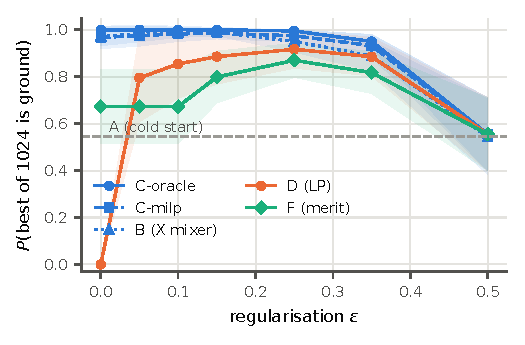
\includegraphics[width=\columnwidth]{figures/fig_eps.pdf}
\caption{$P_{\KMax}$ against the regularisation $\varepsilon$ ($p=1$, L2): structural-group means with 95\% $t$-bands ($n=\NGroupsGL$). At $\varepsilon=\EpsMax$ every warm start reduces to the uniform state.}
\label{fig:eps}
\end{figure}

\begin{figure}[t]
\centering
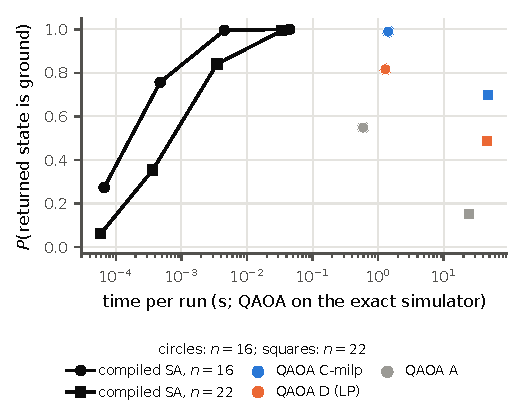
\includegraphics[width=\columnwidth]{figures/fig_classical.pdf}
\caption{Probability that the returned state is an exact ground state against measured time per run: compiled simulated annealing at four budgets vs.\ QAOA (best of \KMax{} samples, exact simulation), at $n=\NLtwo$ (circles) and $n=\NLfour$ (squares).}
\label{fig:classical}
\end{figure}

\section{Future work}

The most useful next step is a computable proxy for wrong pins or for band share, such as the confidence of the learned predictor or the LP's count of near-fractional pins, which would make the diagnostic a design criterion. Beyond that: runs on hardware, where shot and gate noise act together; larger systems and deeper circuits; a full $\varepsilon$ sweep at \NLfour\ qubits; MaxCut at sizes above the ceiling; and problem classes with dense low-energy bands other than unit commitment, to find what separates the cases where band share adds to overlap from those where it does not.

\end{document}
